\section{Вопросы из билетов}

\subsection{Теорема об однозначном представлении булевой функции многочленом Жегалкина.}
\textbf{Теорема (Жегалкина):} Каждая булева функция единственным образом представляется в виде полинома Жегалкина.

$\blacktriangle$ Заметим, что различных булевых функций от $n$ переменных $2^{2^n}$ штук. При этом конъюнкций вида $x_{i_1}\ldots x_{i_k}$ существует ровно $2^n$, так как из $n$ возможных сомножителей каждый или входит в конъюнкцию, или нет. В полиноме у каждой такой конъюнкции стоит 0 или 1, то есть существует $2^{2^n}$ различных полиномов Жегалкина от $n$ переменных.

Теперь достаточно лишь доказать, что различные полиномы реализуют различные функции. Предположим противное. Тогда приравняв два различных полинома и перенеся один из них в другую часть равенства, получим полином, тождественно равный нулю и имеющий ненулевые коэффициенты. Тогда рассмотрим слагаемое с единичным коэффициентом наименьшей длины, то есть с наименьшим числом переменных, входящих в него (любой один, если таких несколько). Подставив единицы на места этих переменных и нули на места остальных, получим, что на этом наборе только одно это слагаемое принимает единичное значение, то есть нулевая функция на одном из наборов принимает значение 1. Противоречие. Значит, каждая булева функция реализуется полиномом Жегалкина единственным образом. $\quad \blacksquare$ 

\subsection{Теорема о дедукции для исчисления высказываний.}

\textbf{Теорема о дедукции:} Пусть $\Gamma$, $A$ -- это $\Gamma \,\cup\, \{A\}$, тогда верно:
$$\frac{\Gamma\vdash A\to B}{\Gamma,A\vdash B}\;\;\Updownarrow$$

$\blacktriangle$ $(\,\Downarrow)$ Пусть $\Gamma \vdash A\to B$, тогда $\Gamma, A \vdash A,\; A\to B$. К выводу применим MP: $A,\;A\to B \vdash B$. Тогда по транзитивности $\Gamma, A\vdash B$. \newline $(\,\Uparrow)$ Доказывается индукцией по длине вывода $B$ из $\Gamma, A$
\begin{itemize}
    \item[(1)] Если этот вывод -- длины $1$, то $B$ -- аксиома или гипотеза (т.е. формула из $\Gamma$). \newline Если B -- аксиома, то имеем вывод $A \to B$ (из $\emptyset$): \newline 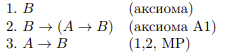
\includegraphics[width=0.35\linewidth]{images/1.1_case1.png}
    \item[(2)] Если $B \in \Gamma$, то имеем такой же вывод $A \to B$ из $\Gamma$: \newline 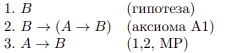
\includegraphics[width=0.35\linewidth]{images/1.1_case2.png}
    \item[(3)] Если $B = A$, то $A \to B = A \to A$. Но $\vdash A \to A$ (пример из определений \ref{a_to_a}).
    \item[(4)] Предположим теперь, что $\Gamma, A \vdash B$ и утверждение $(\,\Uparrow)$ верно для всех более коротких выводов, т.е. для всех $C$, если $\Gamma, A \vdash C$ и вывод $C$ из $\Gamma$, $A$ короче, чем вывод $B$, то $\Gamma$ $\vdash A \to C$.
    \newline Покажем, что $\Gamma \vdash A \to B$. Рассмотрим вывод из $\Gamma, A$, который заканчивается формулой $B$. При этом $B$ может оказаться аксиомой или гипотезой (тогда все предыдущие формулы для доказательства $B$ не нужны). Но в этом случае  $\Gamma \vdash A \to B$ по (1)–(3).
    \newline Остается случай, когда $B$ получается по MP из формул $C, C \to B$, причем $\Gamma, A \vdash C$ и $\Gamma, A \vdash C \to B$ с более короткими доказательствами. По предположению индукции имеем:
    \\
    \\
    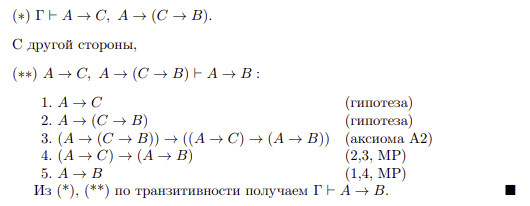
\includegraphics[width=0.8\linewidth]{images/1.1_case3.png}
\end{itemize}

\subsection{Теорема о полноте исчисления высказываний.}

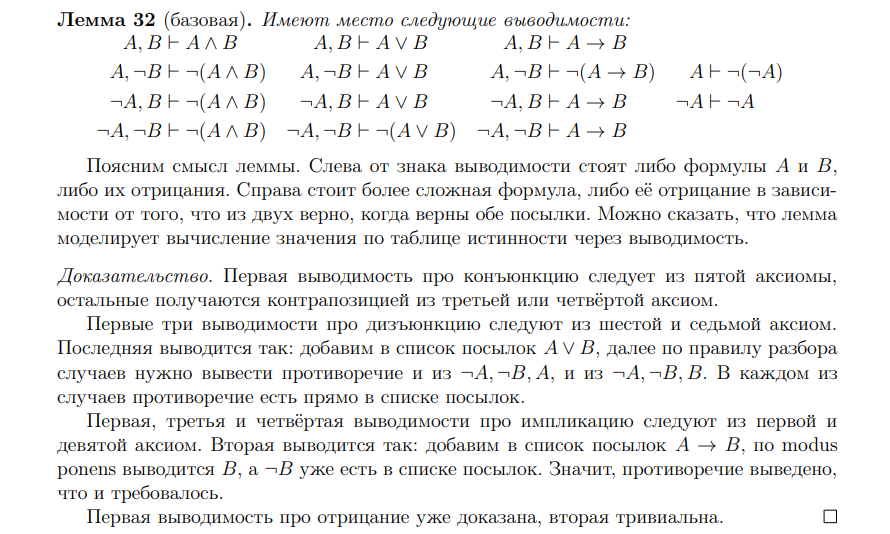
\includegraphics[width=0.93\linewidth]{images/lem_1_base.png}

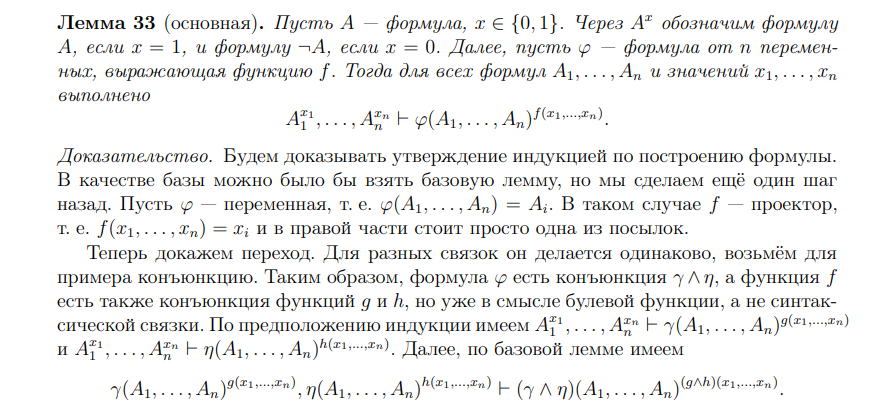
\includegraphics[width=0.93\linewidth]{images/lem_2_main_1.png}

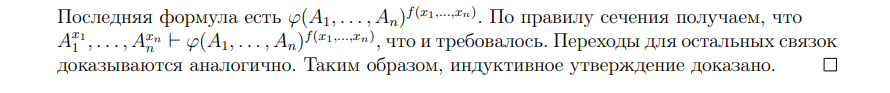
\includegraphics[width=0.93\linewidth]{images/lem_2_main_2.png}

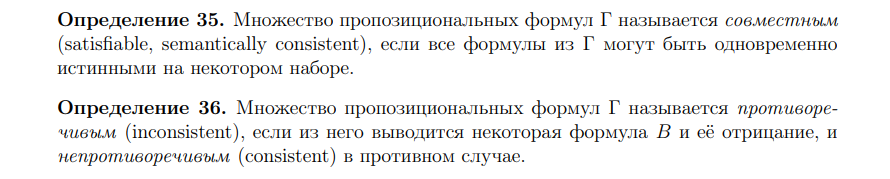
\includegraphics[width=0.93\linewidth]{images/def_for_proof_1.png}

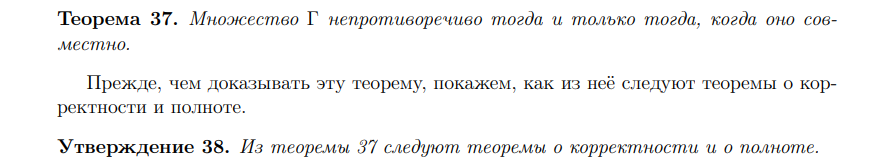
\includegraphics[width=0.93\linewidth]{images/th_main_for_full.png}

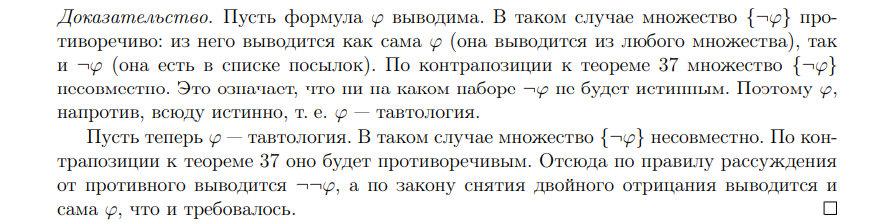
\includegraphics[width=0.93\linewidth]{images/proof_for_prop_1.png}

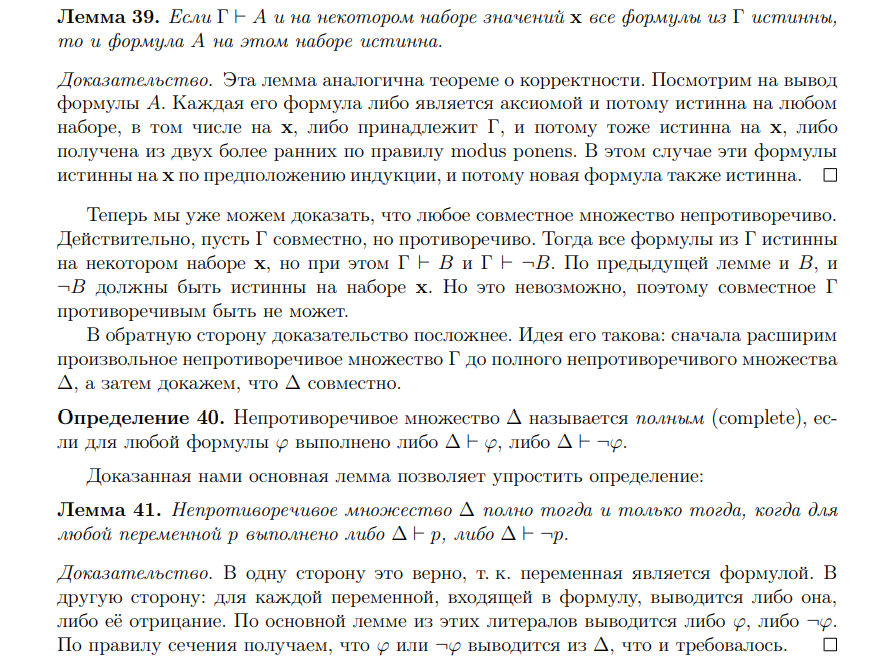
\includegraphics[width=0.93\linewidth]{images/three_lemms_for_full.png}

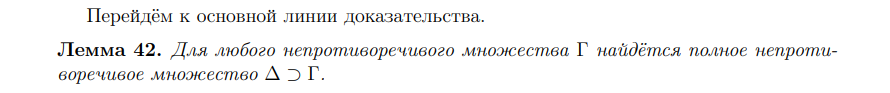
\includegraphics[width=0.93\linewidth]{images/the_last_lemm_full.png}

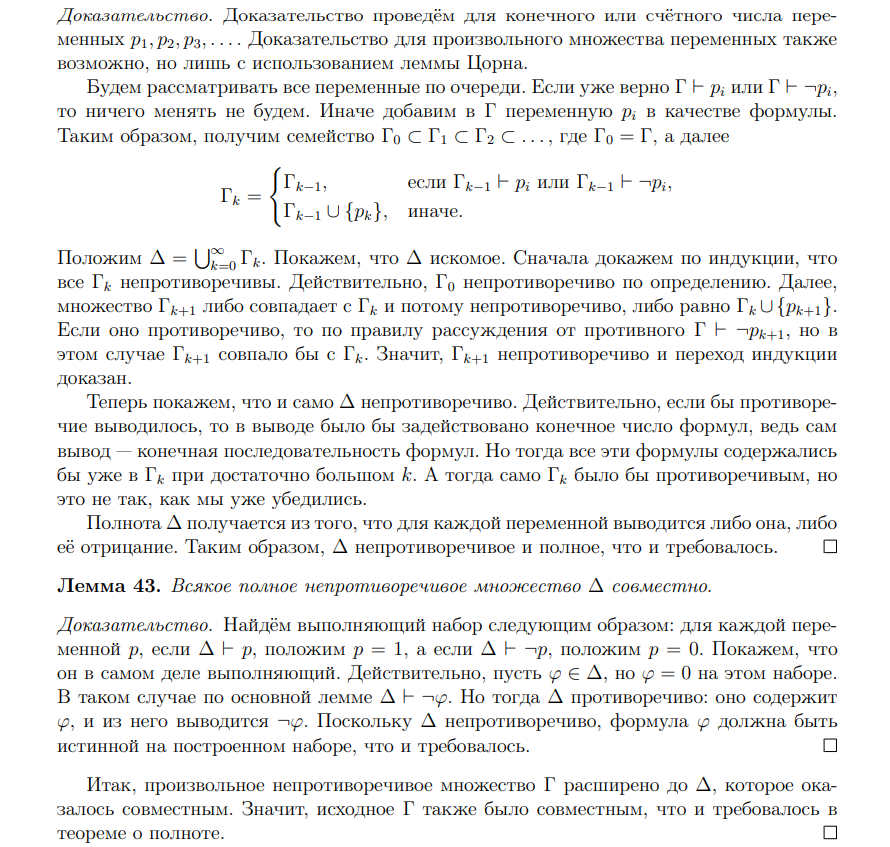
\includegraphics[width=0.93\linewidth]{images/end_of_proof_full.png}


%Из следующей теоремы нам понадобятся только 4) и 6) правила.
%\par

%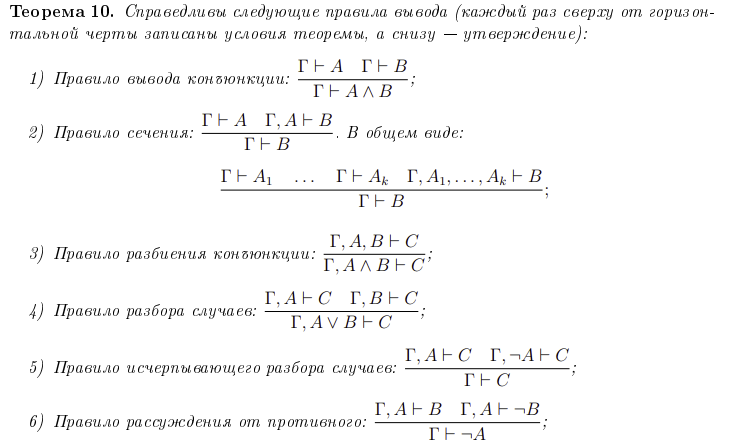
\includegraphics[width=1\linewidth]{images/1.2_theorem}

%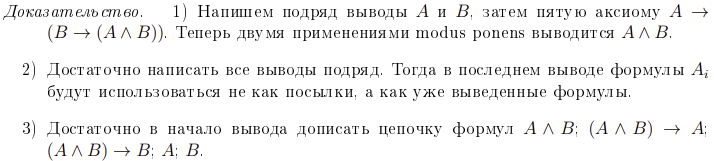
\includegraphics[width=0.97\linewidth]{images/1.1_v1}

%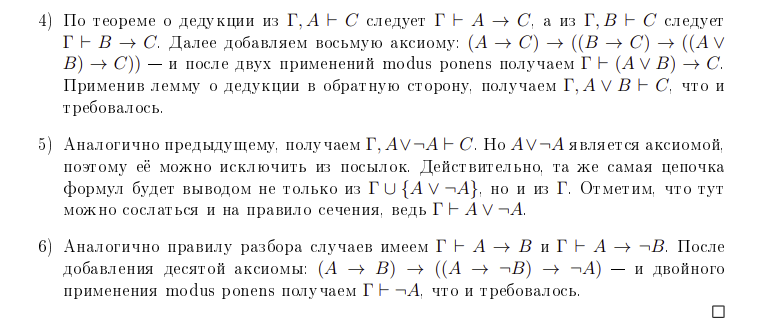
\includegraphics[width=0.97\linewidth]{images/1.1_v3}

%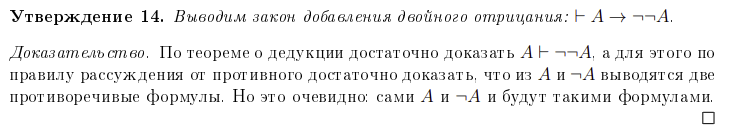
\includegraphics[width=0.97\linewidth]{images/1.1_neg}

%\par \noindent Для доказательства теоремы о полноте понадобятся две вспомогательные леммы.

%\textbf{Базовая лемма:} Представление таблицы истинности для данных четырех связок.

%\begin{tabular}{|p{1.5in}|p{1.5in}|p{1.5in}|p{1.5in}|}
%\hline
%    Для дизъюнкции: & Для конъюнкции: & Для импликации: & Для отрицания:\\ 
%    \hline
%    \centering{$A,B \vdash A\lor B$} & \centering{$A,B \vdash A \land B$} & %\centering{$A,B \vdash A\to B$} & \centering{$A \vdash \neg (\neg A)$} \tabularnewline
%    
%    \centering{$\neg A,B \vdash A\lor B$} & \centering{$\neg A,B \vdash \neg (A\land B)$} & \centering{$\neg A,B \vdash A\to B$}& \centering{$\neg A \vdash \neg A$} \tabularnewline
    
%    \centering{$A,\neg B \vdash A\lor B$} & \centering{$A, \neg B \vdash \neg (A\land B)$} & \centering{$A,\neg B \vdash \neg (A\to B)$}& \centering{} \tabularnewline
    
%    \centering{$\neg A,\neg B \vdash \neg (A\lor B)$} & \centering{$\neg A, \neg B \vdash \neg (A\land B)$} & \centering{$\neg A,\neg B \vdash A\to B$}& \centering{} \tabularnewline
%    \hline
%\end{tabular}

%\begin{enumerate}
%    \item Первые три выводимости про дизъюнкцию следуют из $A_6$ и $A_7$ по лемме о дедукции ($D$). Последняя: \newline
%    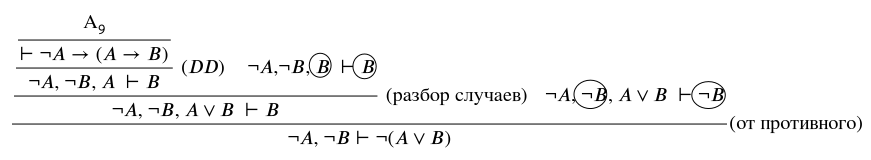
\includegraphics[width=0.99\linewidth]{images/1.1_dedu.png}
%    \item Первая выводимость про конъюнкцию следует из $A_5$ по $D$, остальные получаются контрапозицией из $A_3$ и $A_4$: \newline
%    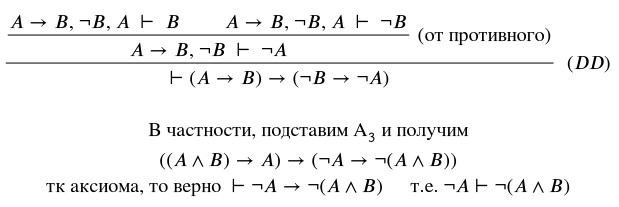
\includegraphics[width=0.8\linewidth]{images/1.1_cntrl.png}
%    \item Первая, третья и четвертая выводимость про импликацию следуют из $A_1$ и $A_9$ по $D$. Вторая выводится так: \newline
%    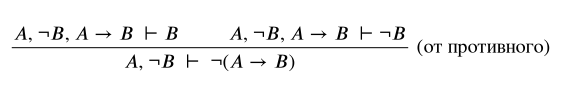
\includegraphics[width=0.7\linewidth]{images/1.1_negg.png}
%    \item Первая выводимость про отрицание доказана в утверждении 14, вторая тривиальна.
%\end{enumerate}

%\par \textbf{Основная лемма:} Пусть $\phi$ - это формула, зависящая от $p_1,\ldots,p_n$. Тогда верно следующее:
%$$p_1^{a_1},p_2^{a_2},\ldots,p_n^{a_n} \vdash \phi^{\phi(a_1,\ldots,a_n)} \text{, \qquad %где } p^a = \begin{cases}
%p, a = 1\\
%\neg p, a = 0
%\end{cases}$$
%Обозначим $a = \phi(a_1,\ldots,a_n)$

%$\blacktriangle$ Доказательство будет вестись индукцией по построению формулы с использованием базовой леммы в качестве базы и в переходе.
%\newline \textit{База индекции:} $\phi$ содержит  одну связку. Тогда это утверждение сводится к базовой лемме.
%\newline \textit{Переход:} пусть $\phi = \psi \land \gamma$. Тогда можно записать: $\phi(a_1,\ldots,a_n) = \psi(a_1,\ldots,a_n) \land \gamma(a_1,\ldots,a_n)$
%\newline Пусть $\psi(a_1,\ldots,a_n) = \alpha, \;\; \gamma(a_1,\ldots,a_n) = \beta$
%\newline Применим предположение индукции: $p_1^{a_1},\ldots,p_n^{a_n} \vdash \psi^\alpha, \;\;\; p_1^{a_1},\ldots,p_n^{a_n} \vdash \gamma^\beta$
%\newline Воспользуемся базовой леммой:
%$\psi^\alpha, \; \gamma^\beta \vdash (\psi \land \gamma)^{(\alpha\land\beta)}=\phi^a $
%\newline Записав все выводы подряд, получаем: $p_1^{a_1},p_2^{a_2},\ldots,p_n^{a_n} \vdash \phi^{a}$
%\newline Аналогичные действия проделаем и для других связок. Имеются база и переход, значит, по индукции докажем лемму для всех формул. $\qquad \blacksquare$

%\textit{Пример:} $\phi=\neg p \land (q\lor r); \quad \phi(0,1,0)=1;\quad \phi(1,0,0)=1$

%Лемма утверждает следующее: $\quad \neg p, q, \neg r \vdash \phi; \qquad p, \neg q, \neg r \vdash \neg \phi$
%\newline \par \textbf{Теорема о полноте ИВ:} Если формула $\phi$ является тавтологией, то тогда $\phi$ -- выводима. 

%$\blacktriangle$ Пусть $\phi$ -- тавтология. Тогда $\forall a_1\ldots a_n \;\; \phi(a_1,\ldots,a_n) = 1$. Значит, по основной лемме $ p_1^{a_1},p_2^{a_2},\ldots,p_n^{a_n} \vdash \phi$ при $\forall a_1\ldots a_n$. Далее воспользуемся правилом исчерпывающего разбора случаев, а также закон исключенного третьего: \newline
%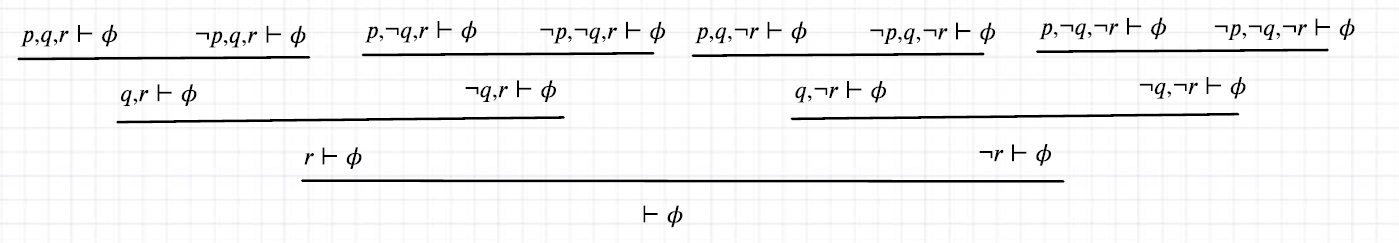
\includegraphics[width=1\linewidth]{images/1.1_cases.png}
%Такое рассуждение можно провести не только для трех литералов, но и для любого количества. Значит, теорема о полноте доказана. $\qquad \blacksquare$



\subsection{Теорема о полноте метода резолюций: из невыполнимой КНФ всегда можно вывести $\perp$.}

\textbf{Теорема.} Метод резолюций всегда заканчивает свою работу, причём для невыполнимых КНФ выводится $\perp$ (полнота), а для выполнимых не выводится (корректность).

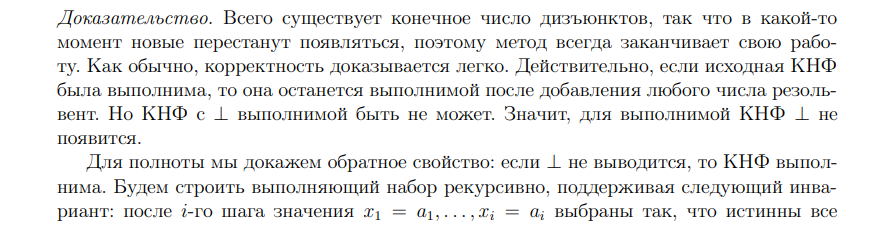
\includegraphics[width=0.95\textwidth]{images/resolut_proof_1.png}

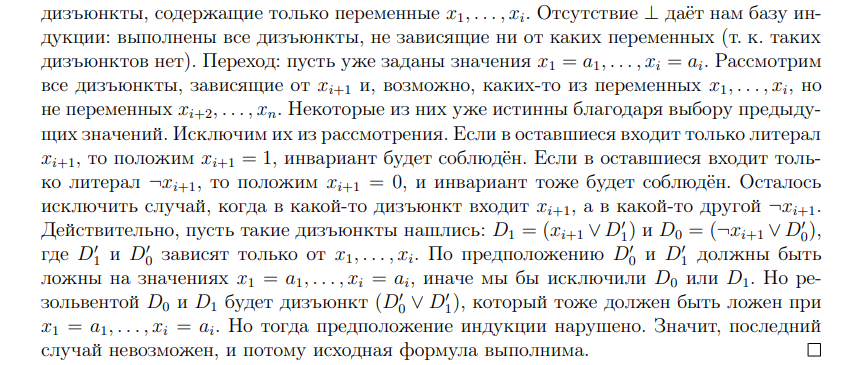
\includegraphics[width=0.95\textwidth]{images/resolut_proof_2.png}


\subsection{Теорема о компактности для исчисления высказываний.}

\textbf{Теорема:} Пусть любое конечное подмножество множества $\Gamma$ совместно. Тогда и всё множество $\Gamma$ совместно.

$\blacktriangle$ Если всё множество $\Gamma$ несовместно, то оно противоречиво. Но тогда в нём есть конечное противоречивое подмножество. Но тогда оно несовместно, что противоречит условию. $\quad \blacksquare$

\subsection{Устойчивость выразимых предикатов при автоморфизмах интерпретаций.}

Пусть имеется некоторая сигнатура $\sigma$ и интерпретация этой сигнатуры, носителем которой является множество $M$.

\textbf{Определение:} Взаимно однозначное отображение $\alpha: M \to M$ называется \textit{автоморфизмом} интерпретации, если все функции и предикаты, входящие в интерпретацию, устойчивы относительно $\alpha$. При этом k-местный предикат $P$ называется \textit{устойчивым} относительно $\alpha$, если 
\[P(\alpha(m_1), \ldots, \alpha(m_k)) \lra P(m_{1}, \ldots, m_{k})\]
для любых элементов $m_1, \ldots, m_k \in M$. Далее, k-местная функция $f$ называется устойчивой относительно $\alpha$, если
\[f(\alpha(m_{1}), \ldots, \alpha(m_{k})) = \alpha(f(m_{1}, \ldots, m_{k})).\]

\textbf{Теорема:} Любой предикат, выразимый в данной интерпретации, устойчив относительно её автоморфизмов.

$\blacktriangle$ Пусть $\pi$ — некоторая оценка, то есть отображение, ставящее в соответствие всем индивидным переменным некоторые элементы носителя. Через $\alpha \circ \pi$ обозначим оценку, которая получится, если к значению каждой переменной применить отображение $\alpha$; другими словами, $\alpha \circ \pi (\xi) = \alpha(\pi(\xi))$ для любой переменной $\xi$.

Первый шаг состоит в том, чтобы индукцией по построению терма t доказать такое утверждение: значение терма t при оценке $\alpha \circ \pi$ получается применением $\alpha$ к значению терма t при оценке $\pi$: $[t](\alpha \circ \pi) = \alpha([t](\pi))$.

Для переменных это очевидно, а шаг индукции использует устойчивость всех функций интерпретации относительно $\alpha$. Теперь индукцией по построению формулы $\varphi$ легко доказать такое утверждение: $[\varphi](\alpha \circ \pi) = [\varphi](\pi)$.

Мы не будем выписывать эту проверку; скажем лишь, что взаимная однозначность $\alpha$ используется, когда мы разбираем случай кванторов. (В самом деле, если с одной стороны изоморфизма берётся какой-то объект, то взаимная однозначность позволяет взять соответствующий ему объект с другой стороны изоморфизма.)
$\blacksquare$

\subsection{Теорема Гёделя о полноте исчисления предикатов: расширение любого непротиворечивого множества до полного и экзистенциально полного.}

\textbf{Определение:} Множество Г замкнутых формул в сигнатуре называется теорией.

\textbf{Определение:} Интерпретация $M$ сигнатуры $\sigma$ называется моделью теории Г, если все формулы из Г истинны в $M$.

\textbf{Определение:} Теория Г называется совместной, если все формулы из Г могут быть одновременно истинны в некоторой интерпретации.

\textbf{Определение:} Теория Г называется противоречивой, если из нее выводится некоторая формула $\phi$ и ее отрицание $\neg\phi$, и непротиворечивой в противном случае.

\par
\textbf{Теорема Гёделя о полноте исчисления предикатов}:
Если $\varphi$ общезначима, то она выводима в исчислении предикатов.
Пользуясь данной терминологией, можно сформулировать теорему, из которой будет следовать теорема Гёделя.

\textbf{Теорема}: Если теория непротиворечива, то она совместна (имеет модель).

\textbf{Доказательство:} 1. Мы хотим расширить не противоречивую Г так, чтобы она была полной (если $\varphi$ - замкнутая формула, то Г $ \vdash \varphi$ или  Г $ \vdash \neg \varphi$) и экзистенциально полной (т.е. если Г $ \vdash \exists x \varphi$, то Г $ \vdash \varphi(t/x)$, где t - замкнутый терм.
\begin{center}
    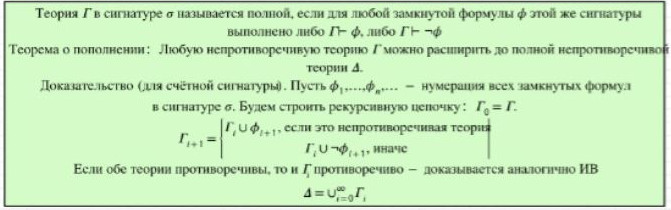
\includegraphics[width=13cm]{images/1.5_m1}

    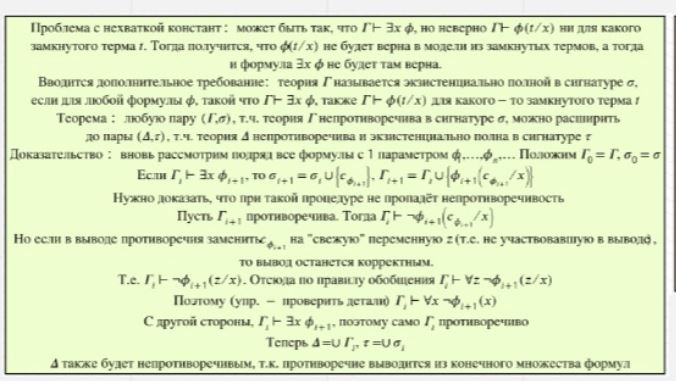
\includegraphics[width=13cm]{images/1.5_m2}

    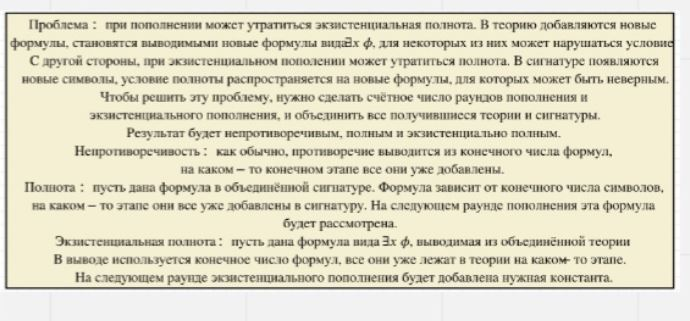
\includegraphics[width=12cm]{images/1.5_m3}

    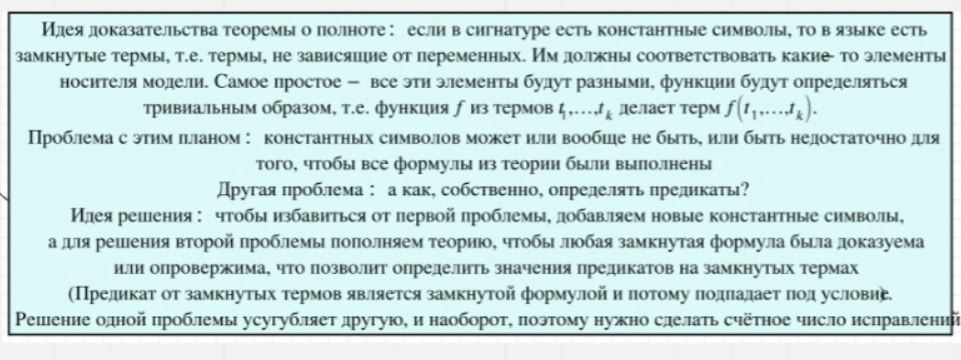
\includegraphics[width=12cm]{images/1.5_full}
\end{center}

\textbf{Лемма 9}.
Любую непротиворечивую теорию можно расширить до непротиворечивой, полной и экзистенциально полной теории.

Доказательство было приведено выше.

\subsection{Теорема Гёделя о полноте исчисления предикатов: построение модели из замкнутых термов у любого непротиворечивого, полного и экзистенциально полного множества.}

\textbf{Лемма 10}.

Любая непротиворечивая, полная, экзистенциально полная теория совместна, то есть имеет модель.
\begin{center}
    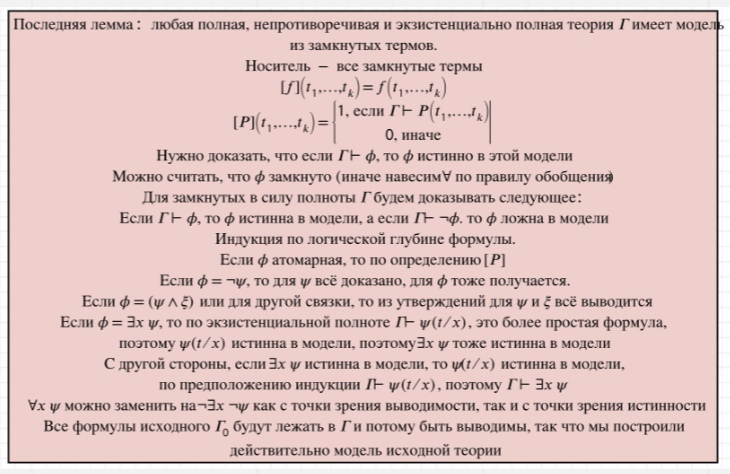
\includegraphics[width=12cm]{images/1.5_full2}    
\end{center}

\subsection{Представимость конечных последовательностей в арифметике при помощи $\beta$-функции Гёделя.}

\textbf{Лемма 1}:\\

$\forall n \quad \forall c \quad \exists b > c$ такое, что $b + 1,  2b + 1, \dotsc, nb + 1$ - взаимно просты.\\

Рассмотрим $b = n!$.

Тогда возьмем произвольные различные $k$ и $m$ от $1$ до $n$. $gcd(kb + 1, mb + 1) = d > 1 \Rightarrow (k - m)b$ делится на $d$.

Значит т.к. $b = n!$ и $k - m < n$, получаем, что любой простой делитель числа $(k - m)b$ должен быть строго меньше $n$.\\

У $d$ есть простой делитель $p < n$.

$mb + 1$ делится на $p$.

$mb + 1 - m\cdot n!$ делится на $p \Rightarrow d = 1$ 
\\

\textbf{Лемма 2.}\\

$\forall (x_1, \dotsc, x_n) \quad\exists a, b \quad \forall i : a \equiv x_i \quad mod (b_i + 1)$\\

\textbf{Док-во:}\\

Выберем по Лемме 1 $b > max\{x_i\}$.\\

Тогда нужное $a$ найдётся по китайской теореме об остатках: Если натуральные числа $a_1, \dotsc, a_n$  попарно взаимно просты, то для любых $r_1, \dotsc, r_n$ таких, что $0 \leq r_i < a_i$ при всех $i : 0, \dotsc, n$ найдется число, которое при делении на $a_i$ дает остаток $r_i$ при всех $i$. Более того, если найдутся два таких числа, то они будут сравнимы по модулю $a_1 \cdot \dotsc \cdot a_n$.\\

Положим $\beta(a, b, i) = a \quad mod (bi + 1)$

$\beta$ арифметична: $r = x \quad mod(q) \Leftrightarrow r < q$ и $\exists s: x = sq + r$.

\subsection{Арифметичность предикатов «n — степень шестёрки» и $n = 2^k$.}

\textbf{Определение:} Предикат $P: \N^k \to \{0,1\}$ называется \textit{арифметичным}, если он выразим в стандартной интерпретации арифметики $\langle \N, +, \cdot, = \rangle$. Функция $f: \mathbb{N}^k \rightarrow \mathbb{N}$ называется \textit{арифметичной}, если арифметичен предикат $P_{f}: \mathbb{N}^{k+1} \rightarrow \{0,1\}$, где $P_f(x,y) = 1 \lra f(x) = y$.
\\
\\
\textbf{Степень шестерки}
\\
Степень шестерки можно выразить с использованием квантора по конечному множеству\\
    $\exists D (x \in D \wedge \forall y \in D (y = 1 \vee (y \ \vdots \ 6 \wedge \frac{y}{6} \in D)))$ \\ У нас есть $x, \frac{x}{6}, \frac{x}{36}, \frac{x}{216}, ..., 1$. Этакий мешок с числами. И если в нем есть х, то есть и $\frac{x}{6}$ и т.д., а остановиться это все может только на единице. Соответственно, если x - не степень шестерки, то возникнет не единица, и оба условия будут нарушены.
    \\
    \\
    Через обычные предикаты эта функция выражается с помощью кодирования Смаллиана. Оно лучше применимо для описания конечных множеств. В чем суть:
    \\
    Берем и вводим предикат $S(a,b,x)$, которые отвечает следующим свойствам:
    \begin{itemize}
        \item [1] $\forall a,b\{x: S(a,b,x) = 1\}$ - конечно
        \item[2] Для любого конечного S найдутся такие a и b, что $S = \{x: S(a,b,x) = 1\}$
    \end{itemize}
    Теперь записанную нами формулу $\exists D .... x \in D....$ можно переписать следующим образом:\\
    $\exists a,\exists b (S(a,b,x) \wedge \forall y(S(a,b,y) \rightarrow (y = 1 \vee(y \ \vdots \ 6 \wedge \exists z(y = 6\cdot z \wedge S(a,b,z))))))$ \\
    Что поменялось? Заменили $\exists D$ на $\exists a, \exists b$. И $x \in D$ на $S(a,b,x)$, получили формулу первого порядка\\\\
\textbf{Степень двойки}\\
$x = 2^k $ можно выразить с использованием квантора по конечной последовательности\\
$\exists \{a_i\} (a_0 = 1 \wedge a_k = x \wedge \forall i \in [0;k-1] \ a_{i+1} = a\cdot a_i)$
\\
\\
Через обычные предикаты это выражается с использованием $\beta$-функции Гёделя. 
\\
Тут вводится арифметическая функция $\beta(a,b,i)$ со следующим свойством:
\begin{itemize}
    \item[] $\forall [x_0, ..., x_n]$ найдутся такие a,b, что $\forall i \in [0,n] \ x_i = \beta(a,b,i)$
\end{itemize}
Теперь в формуле, которая имеет вид $\exists \{x_i\} ......x_j......$ можно заменить на такую: $\exists a \exists b ......\beta(a,b,j)......$
\\
\\
Применим полученные знания к нашему предикату и получим:\\
$x = 2^k \Longleftrightarrow \exists a,b \ (\beta(a,b,0) = 1 \wedge \beta(a,b,k) = x \wedge \forall i \in [0,..., k-1] \ \beta(a,b,i+1) = 2\cdot \beta(a,b,i) $


\subsection{Множество замкнутых формул, истинных в $\mathbb N$, неперечислимо. Первая теорема Гёделя о неполноте.}

\textbf{Опр} Множество A $\subset \mathbb{N}^k$ называется \textit{арифметическим}, если существует арифметическая формула $\alpha$ с параметрами $x_1, . . . , x_k$, которая его представляет в следующем смысле: $<n_1, . . . , n_k>$ принадлежит множеству A тогда и только тогда, когда формула $\alpha$ истинна при значениях параметров $x_1 = n_1, . . . , x_k = n_k$.
\\
\\
Любое перечислимое множество арифметично
\\
\\
\textbf{Лемма1}\\
Всякое арифметическое множество лежит в классе $\Sigma_n$ или $\Pi_n$ для некоторого n (и, естественно, для всех больших n).
\\
$\blacktriangle$ Формулу, задающую арифметическое множество, приведём к предварённой нормальной форме (вынеся кванторы наружу). Ясно, что бескванторная часть задаёт разрешимое множество, поэтому исходное множество принадлежит какому-то из классов $\Sigma_n$ или $\Pi_n$. Можно и не использовать предварённой нормальной формы, а применить индукцию по длине формулы и сослаться на то, что пересечение, объединение и дополнение, а также проекция не выводят за пределы арифметической иерархии (объединения всех классов $\Sigma_n$ и $\Pi_n$). $\blacksquare$
\\
\\
Рассмотрим теперь множество T, элементами которого являются
все истинные арифметические формулы без параметров (точнее, их номера в какой-то вычислимой нумерации всех формул — это значит, что по формуле можно алгоритмически получить её номер и наоборот).
\\
\\
\textbf{Лемма2}\\ Любое арифметическое множество m-сводится к множеству T.\\
$\blacktriangle$ Пусть A — произвольное арифметическое множество. Пусть $\alpha$(x) — формула с одной переменной, которая выражает принадлежность множеству A. Это означает, что $\alpha$(n) истинно при тех и только тех n, которые принадлежат A.
Тогда вычислимая функция n $\rightarrow$ (номер формулы, которая является
результатом подстановки константы n в $\alpha$(x)) m-сводит A к T. $\blacksquare$
\\
\\
\textbf{ Первая теорема
Гёделя о неполноте}\\
Множество T арифметических истин неперечислимо.\\
$\blacktriangle$ Это следует из того, что если бы Т было перечислимо, оно было бы арифметично, что противоречит теореме Тарского $\blacksquare$ 
\\
\\
\textbf{Множество замкнутых формул, истинных в N, неперечислимо } \\
Если множество перечислимо, то оно лежит в арифметической иерархии, что противоречит теореме Тарского


\subsection{Теорема Тарского.}

\textbf{Теорема Тарского}\\
Истинность арифметической формулы нельзя выразить арифметическим выражением. То есть не существует формулы True(x), которая истинна тогда и только тогда, когда формула с номером х истинна. (Множество T не арифметично.)
\\
$\blacktriangle$ Если бы T было арифметическим, то оно лежало бы в некотором конкретном классе . Поскольку всякое арифметическое множество сводится к T, то все арифметические множества лежали бы в этом классе. Но мы знаем, что множества из более высоких классов иерархии тоже арифметичны, но в $\Sigma_n$ не лежат.$\blacksquare$